\documentclass{article}

\usepackage{fullpage}
\usepackage{amsmath}
\usepackage{amsthm}
\usepackage{graphics}
\usepackage{graphicx}

\newtheorem{theorem}{Theorem}

\author{Olivier Beaumont, Lionel Eyraud-Dubois, Erik Saule}

\title{Fun with recursivity and parallel graph construction}

\begin{document}

\maketitle

\section{Multiplying Large Integers}

\subsection{Variants}

\subsubsection{Naive}

\subsubsection{Karatsuba}

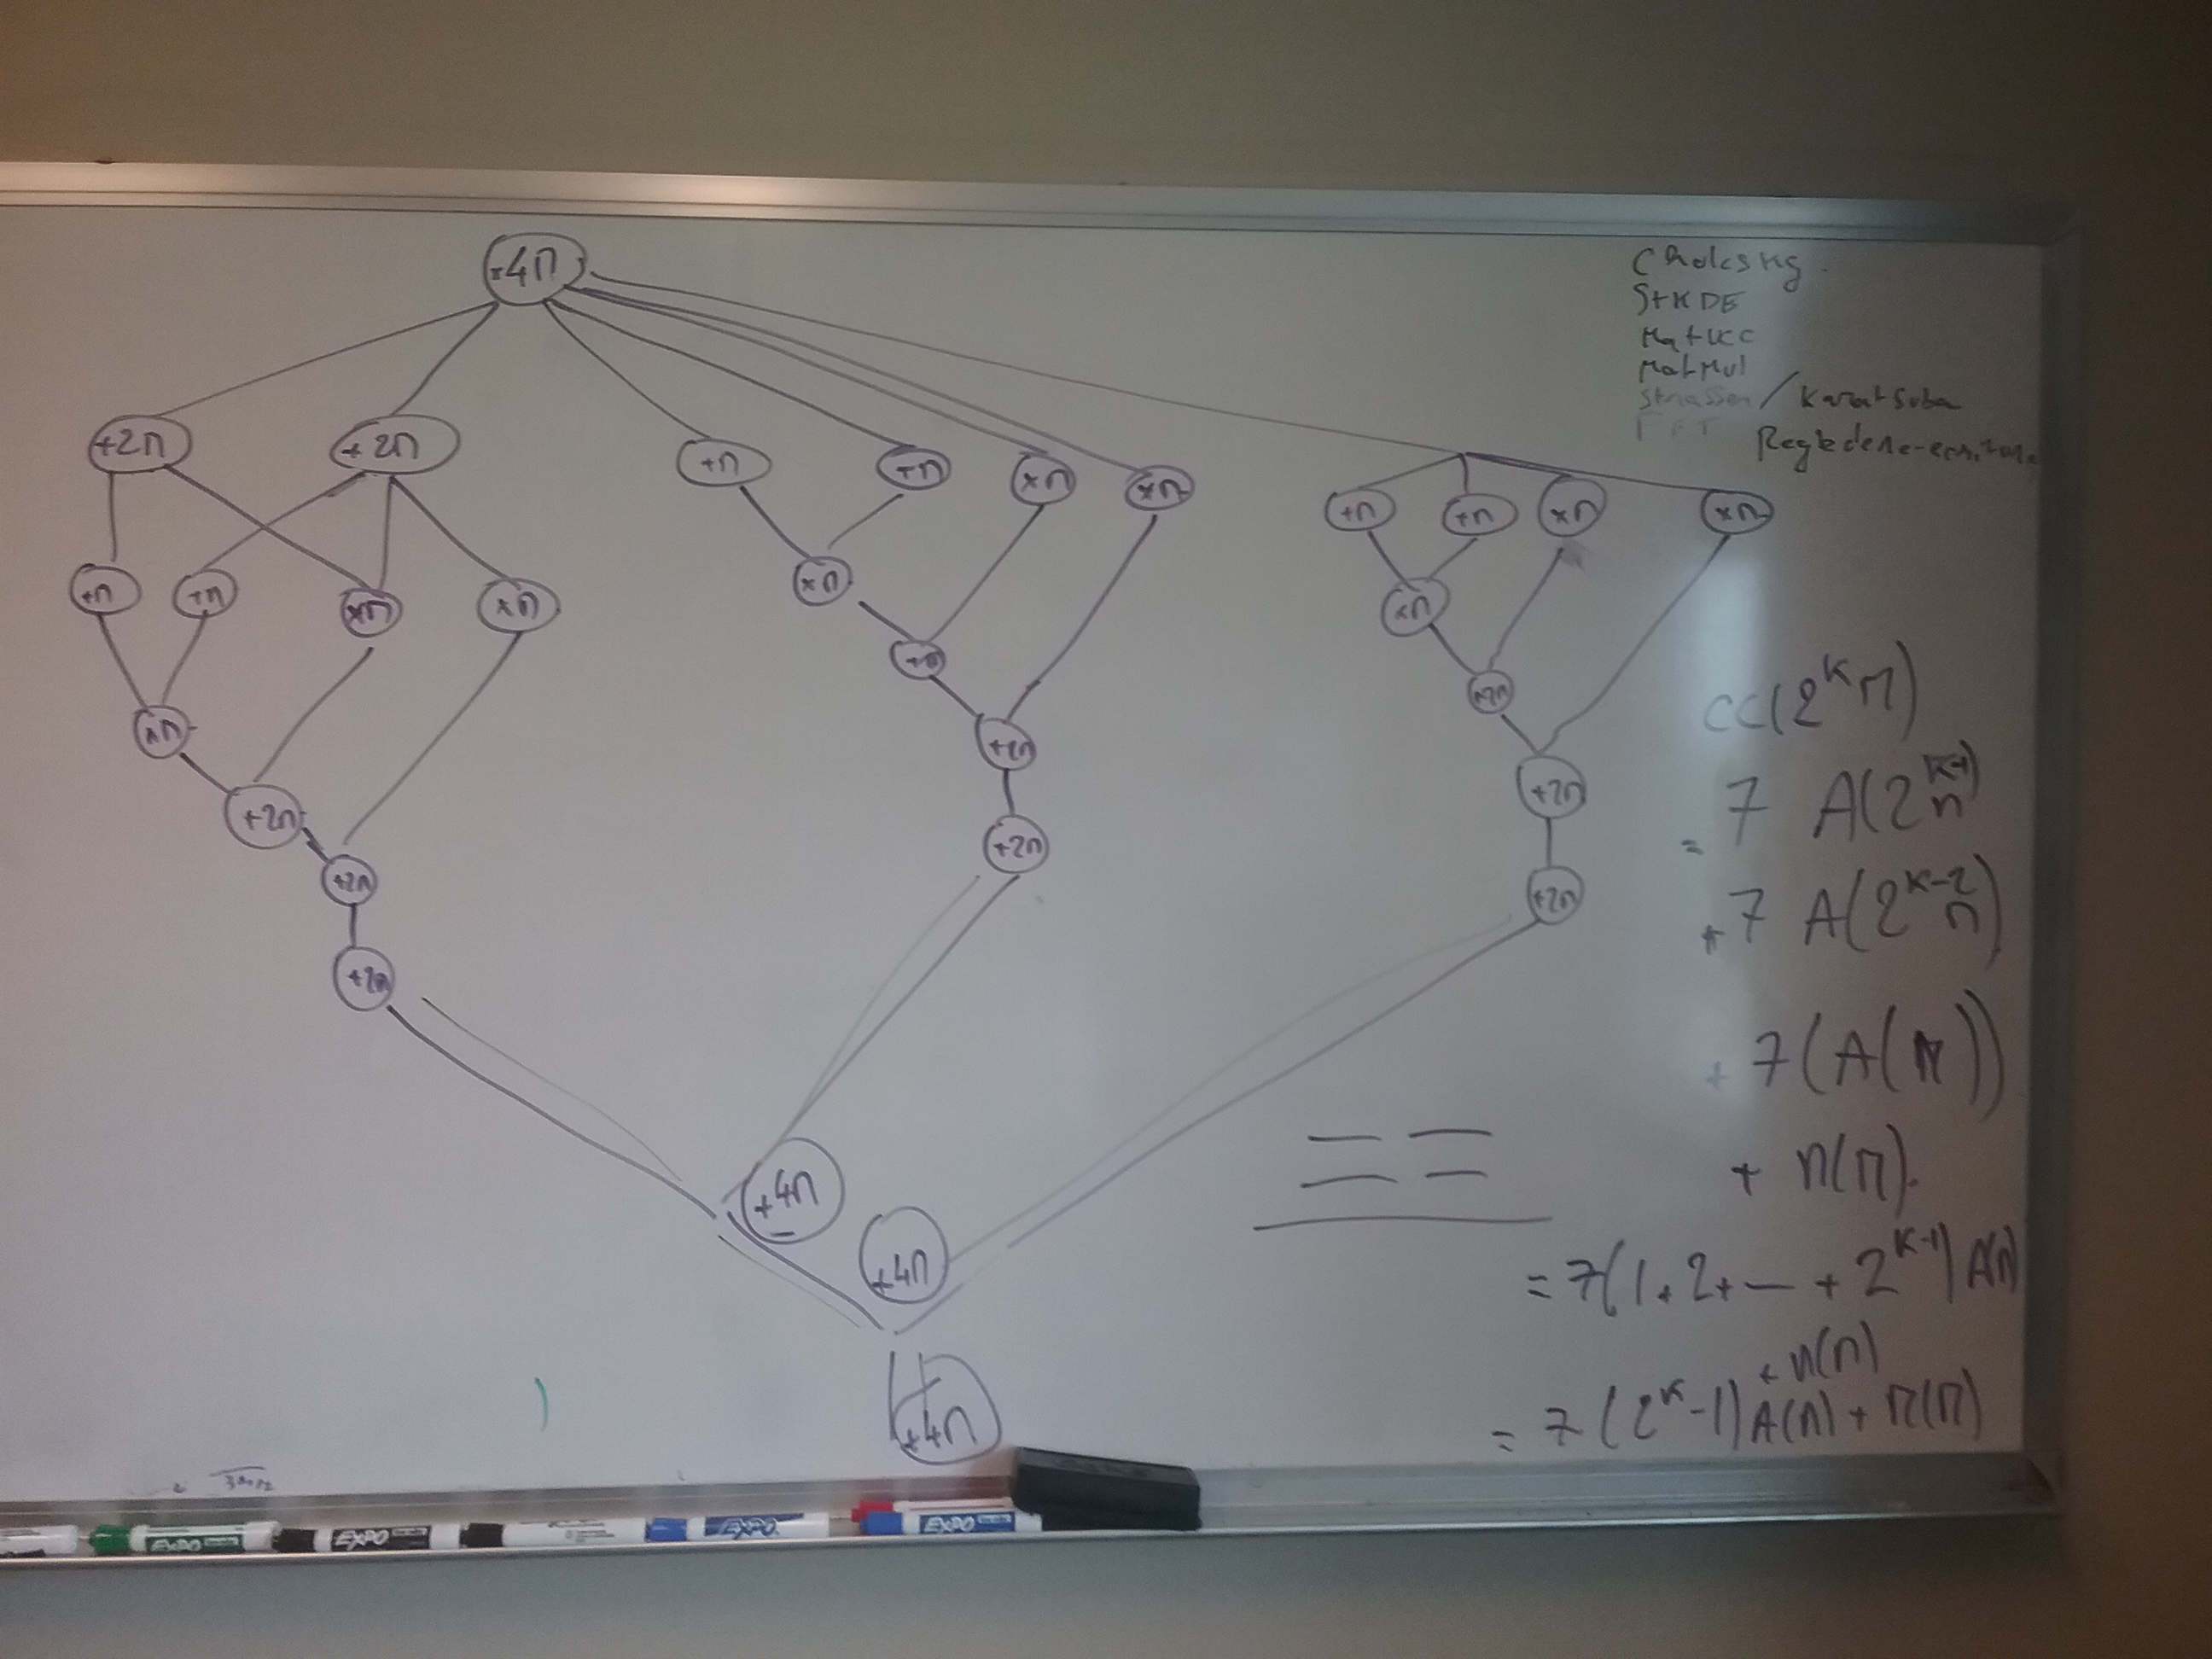
\includegraphics[width=.3\linewidth]{../../notes/20180608_120848.jpg}

\subsection{Hybridization}

\begin{theorem}
Karatsuba at high levels, naive then
\end{theorem}

\begin{proof}
\end{proof}

Analysis: 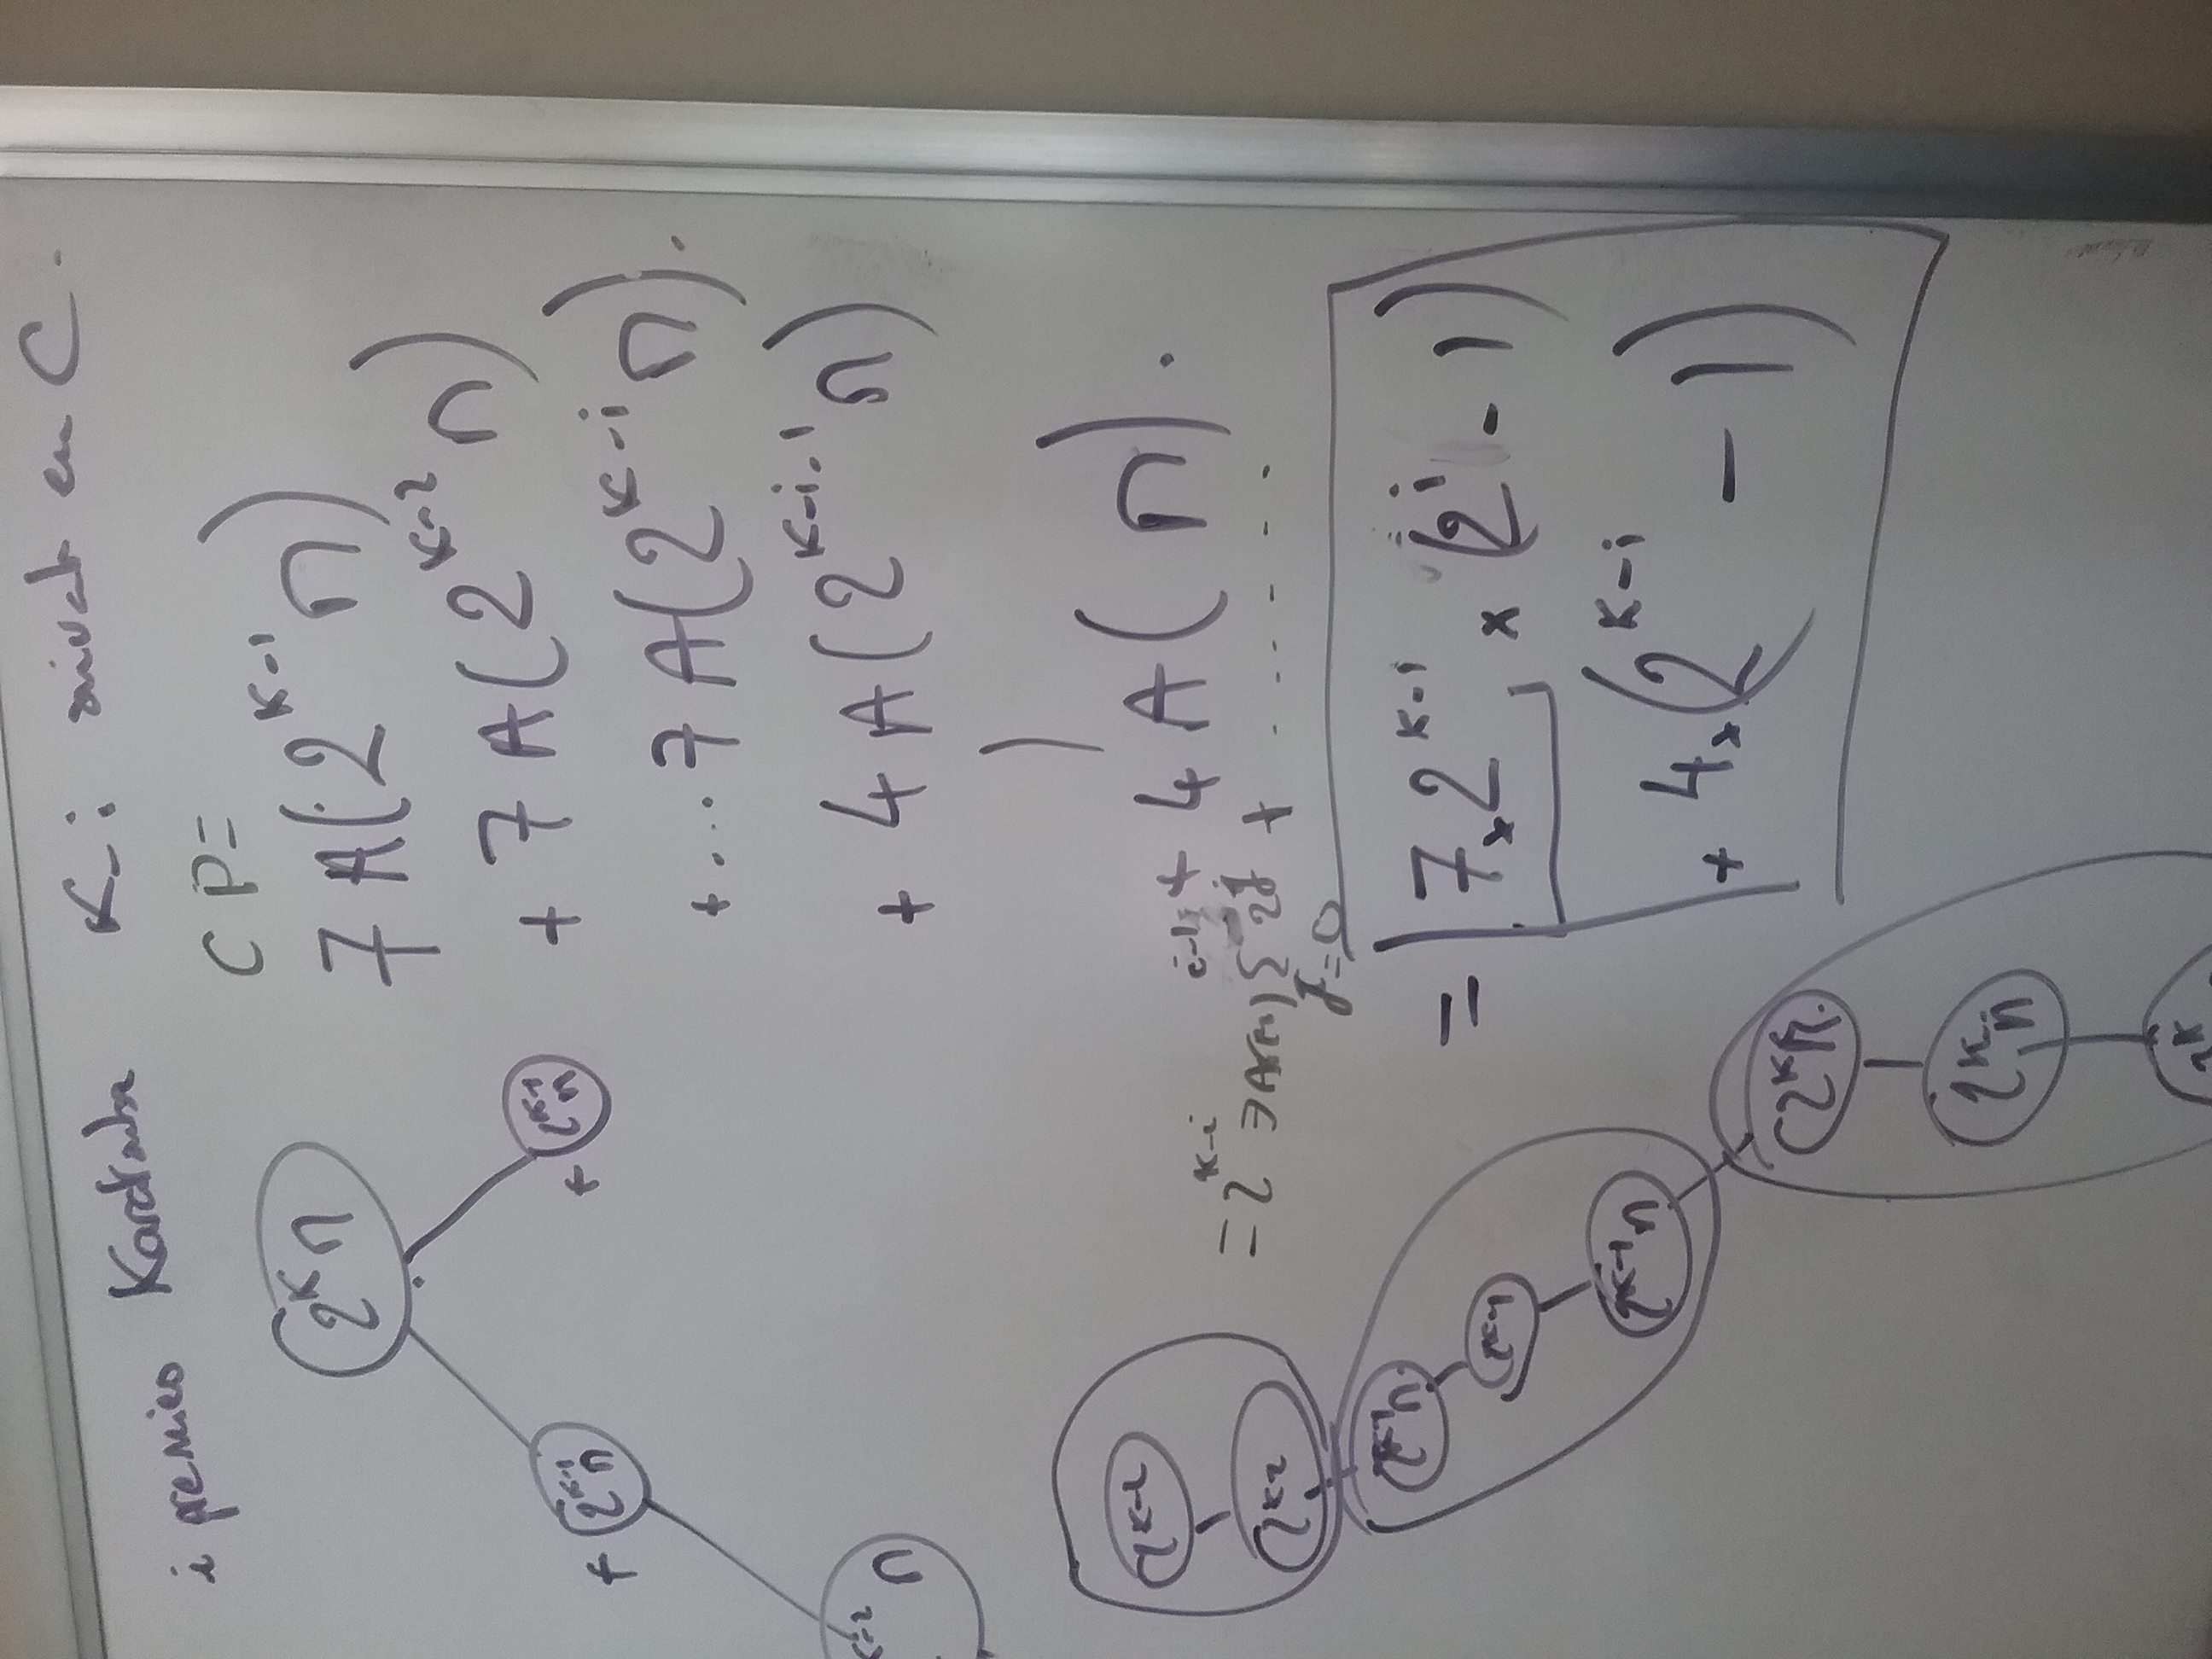
\includegraphics[width=.3\linewidth]{../../notes/20180608_142908.jpg}

\subsection{Generalization}

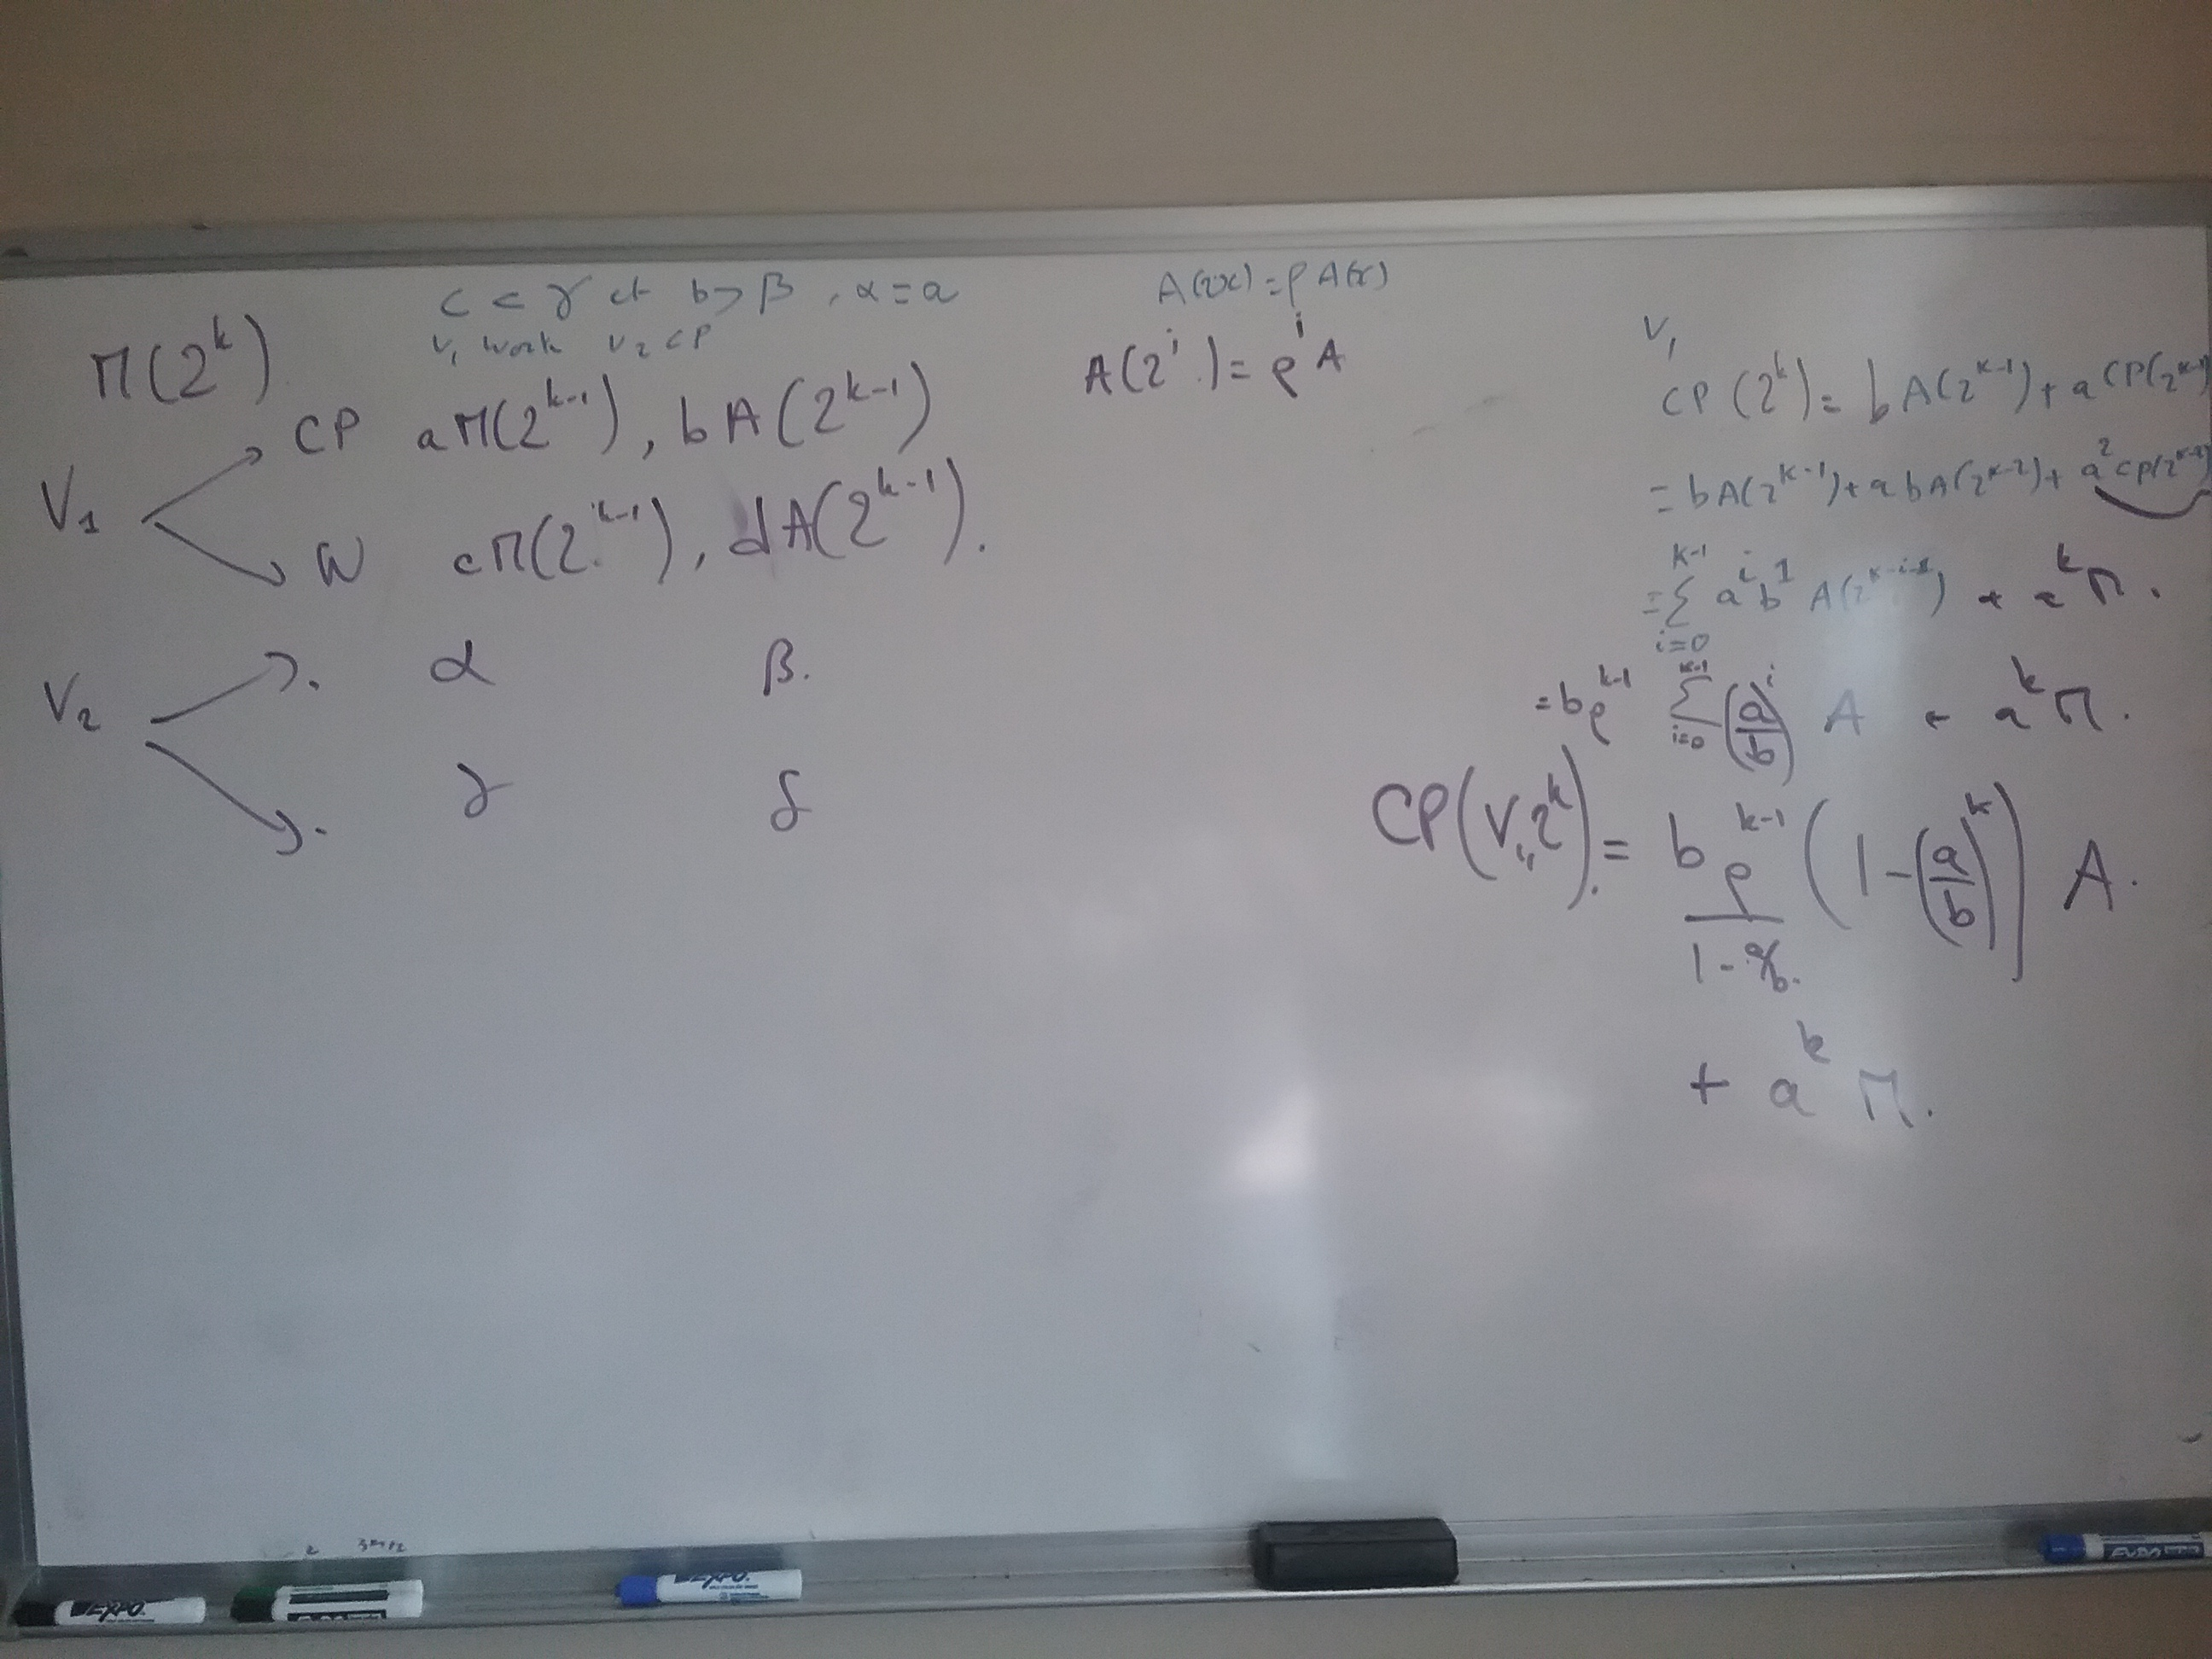
\includegraphics[width=.3\linewidth]{../../notes/20180608_172003.jpg}

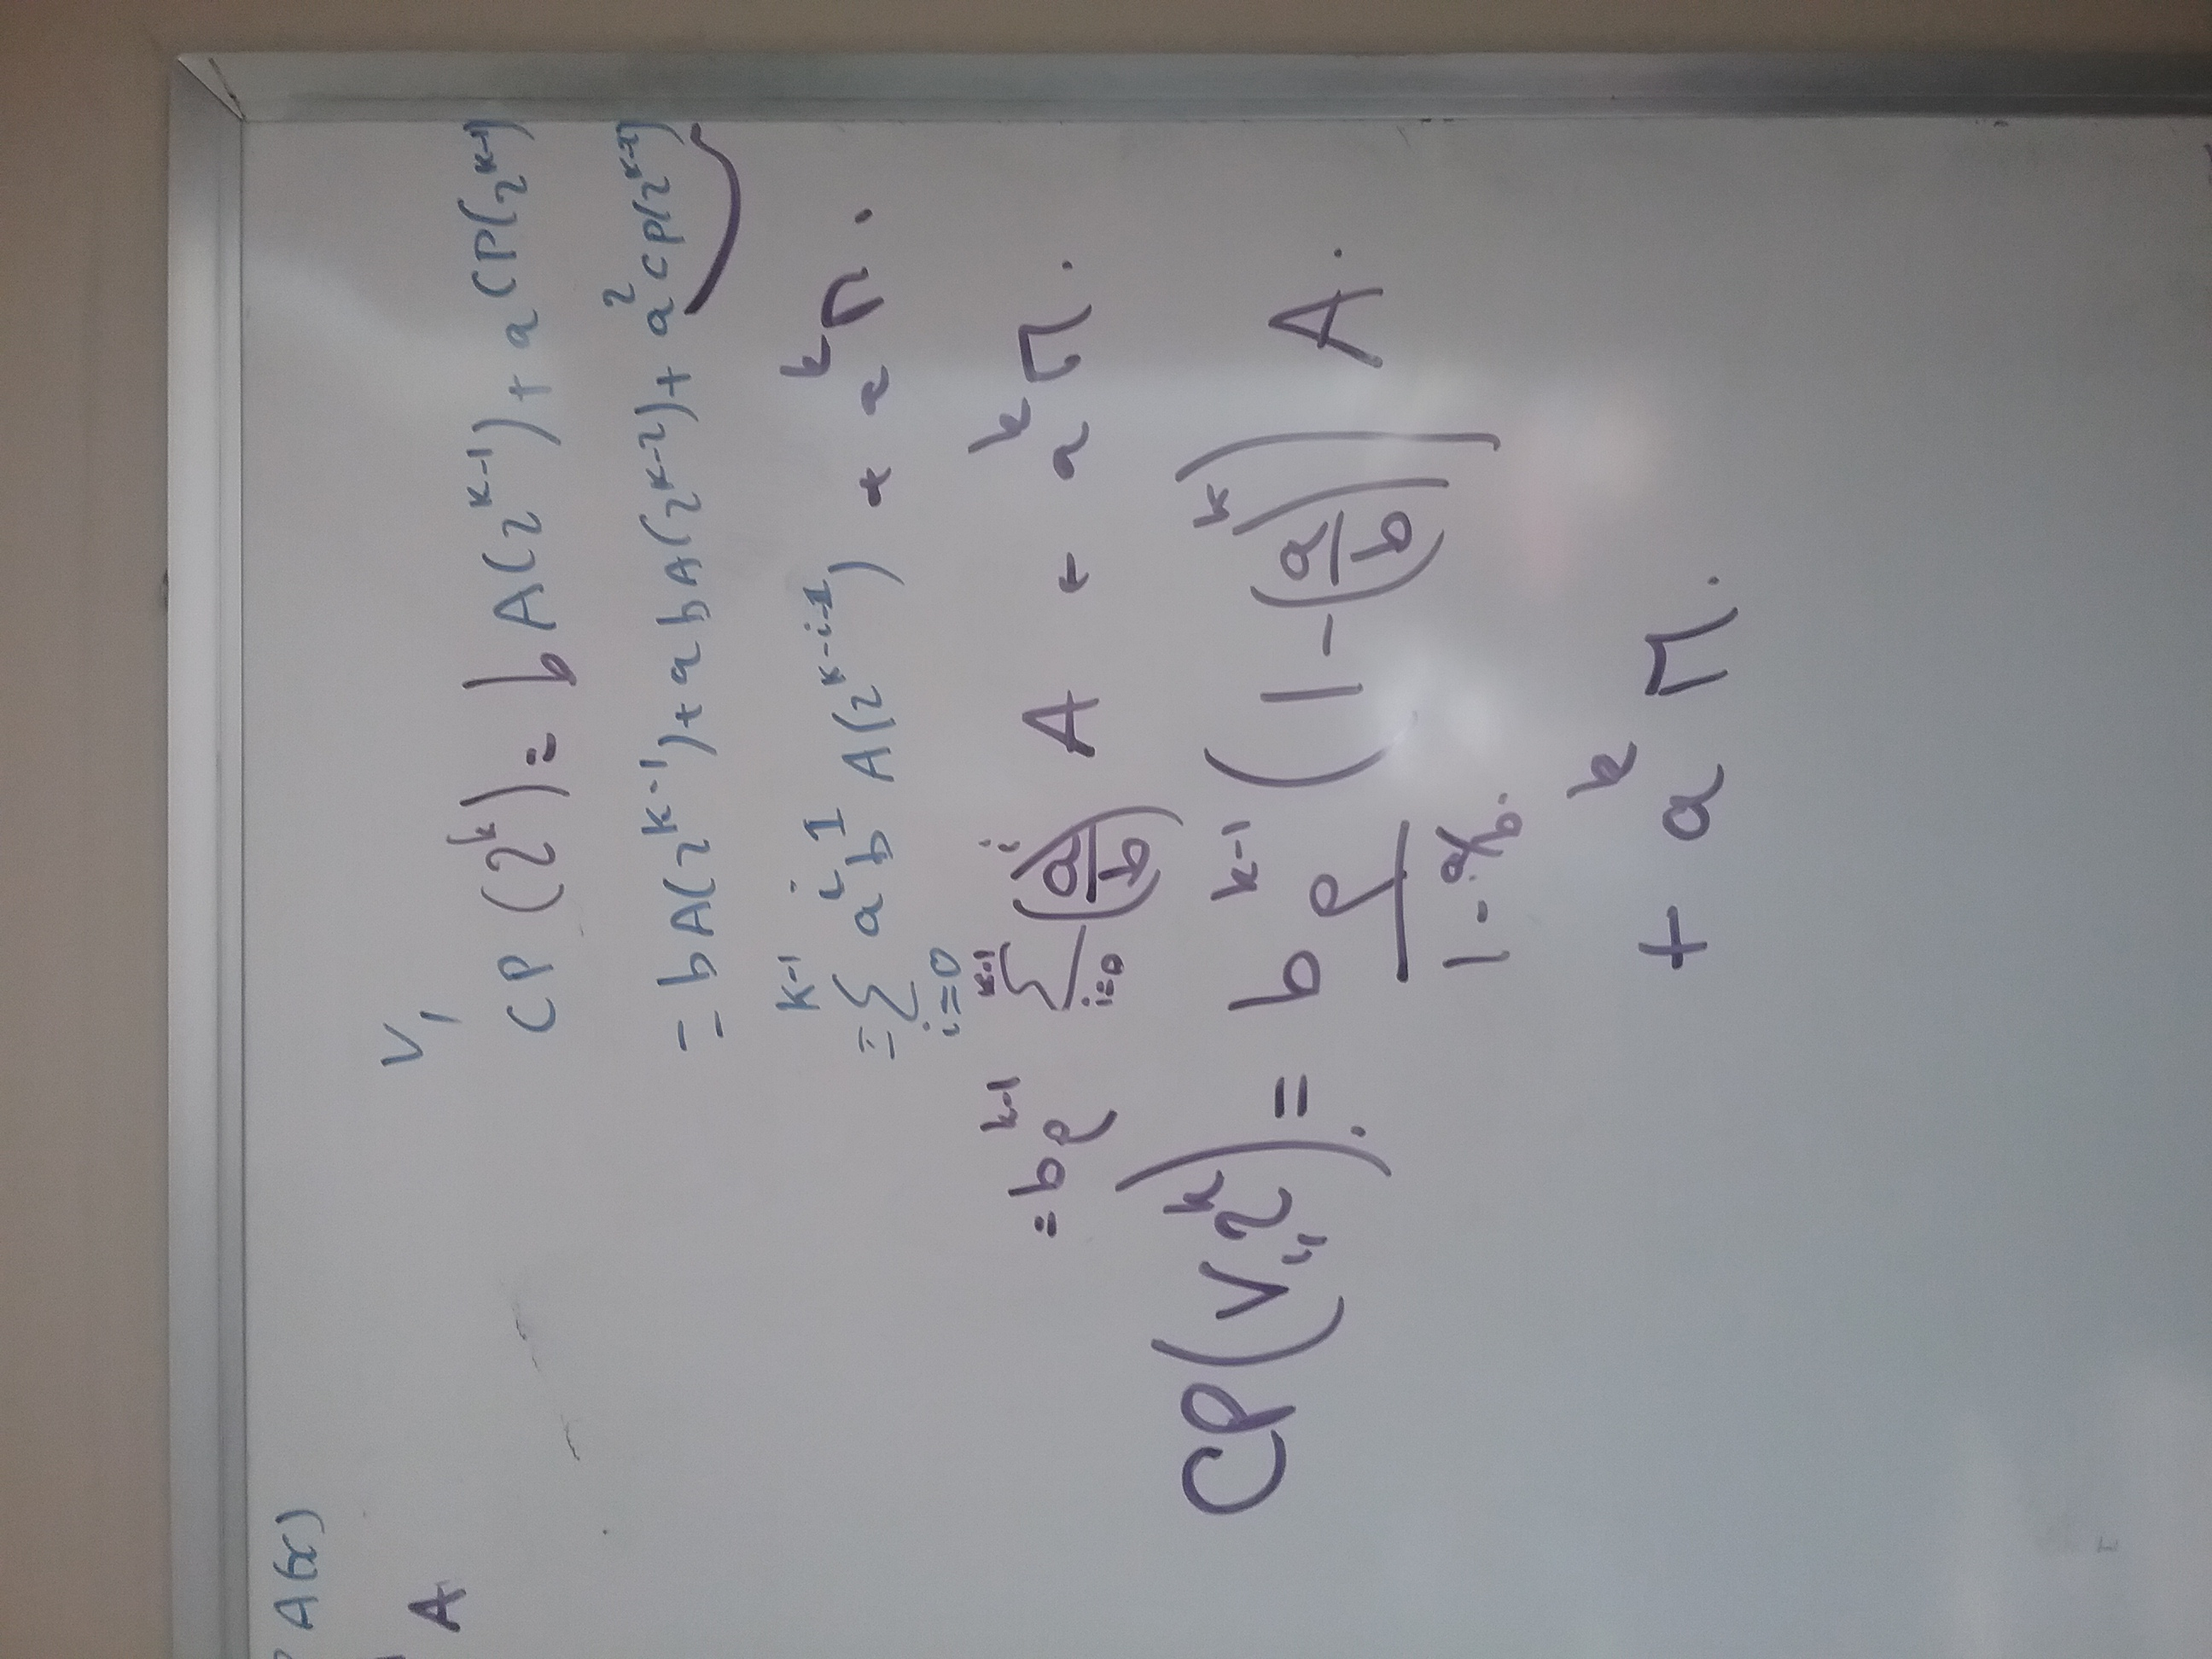
\includegraphics[width=.3\linewidth]{../../notes/20180608_172007.jpg}

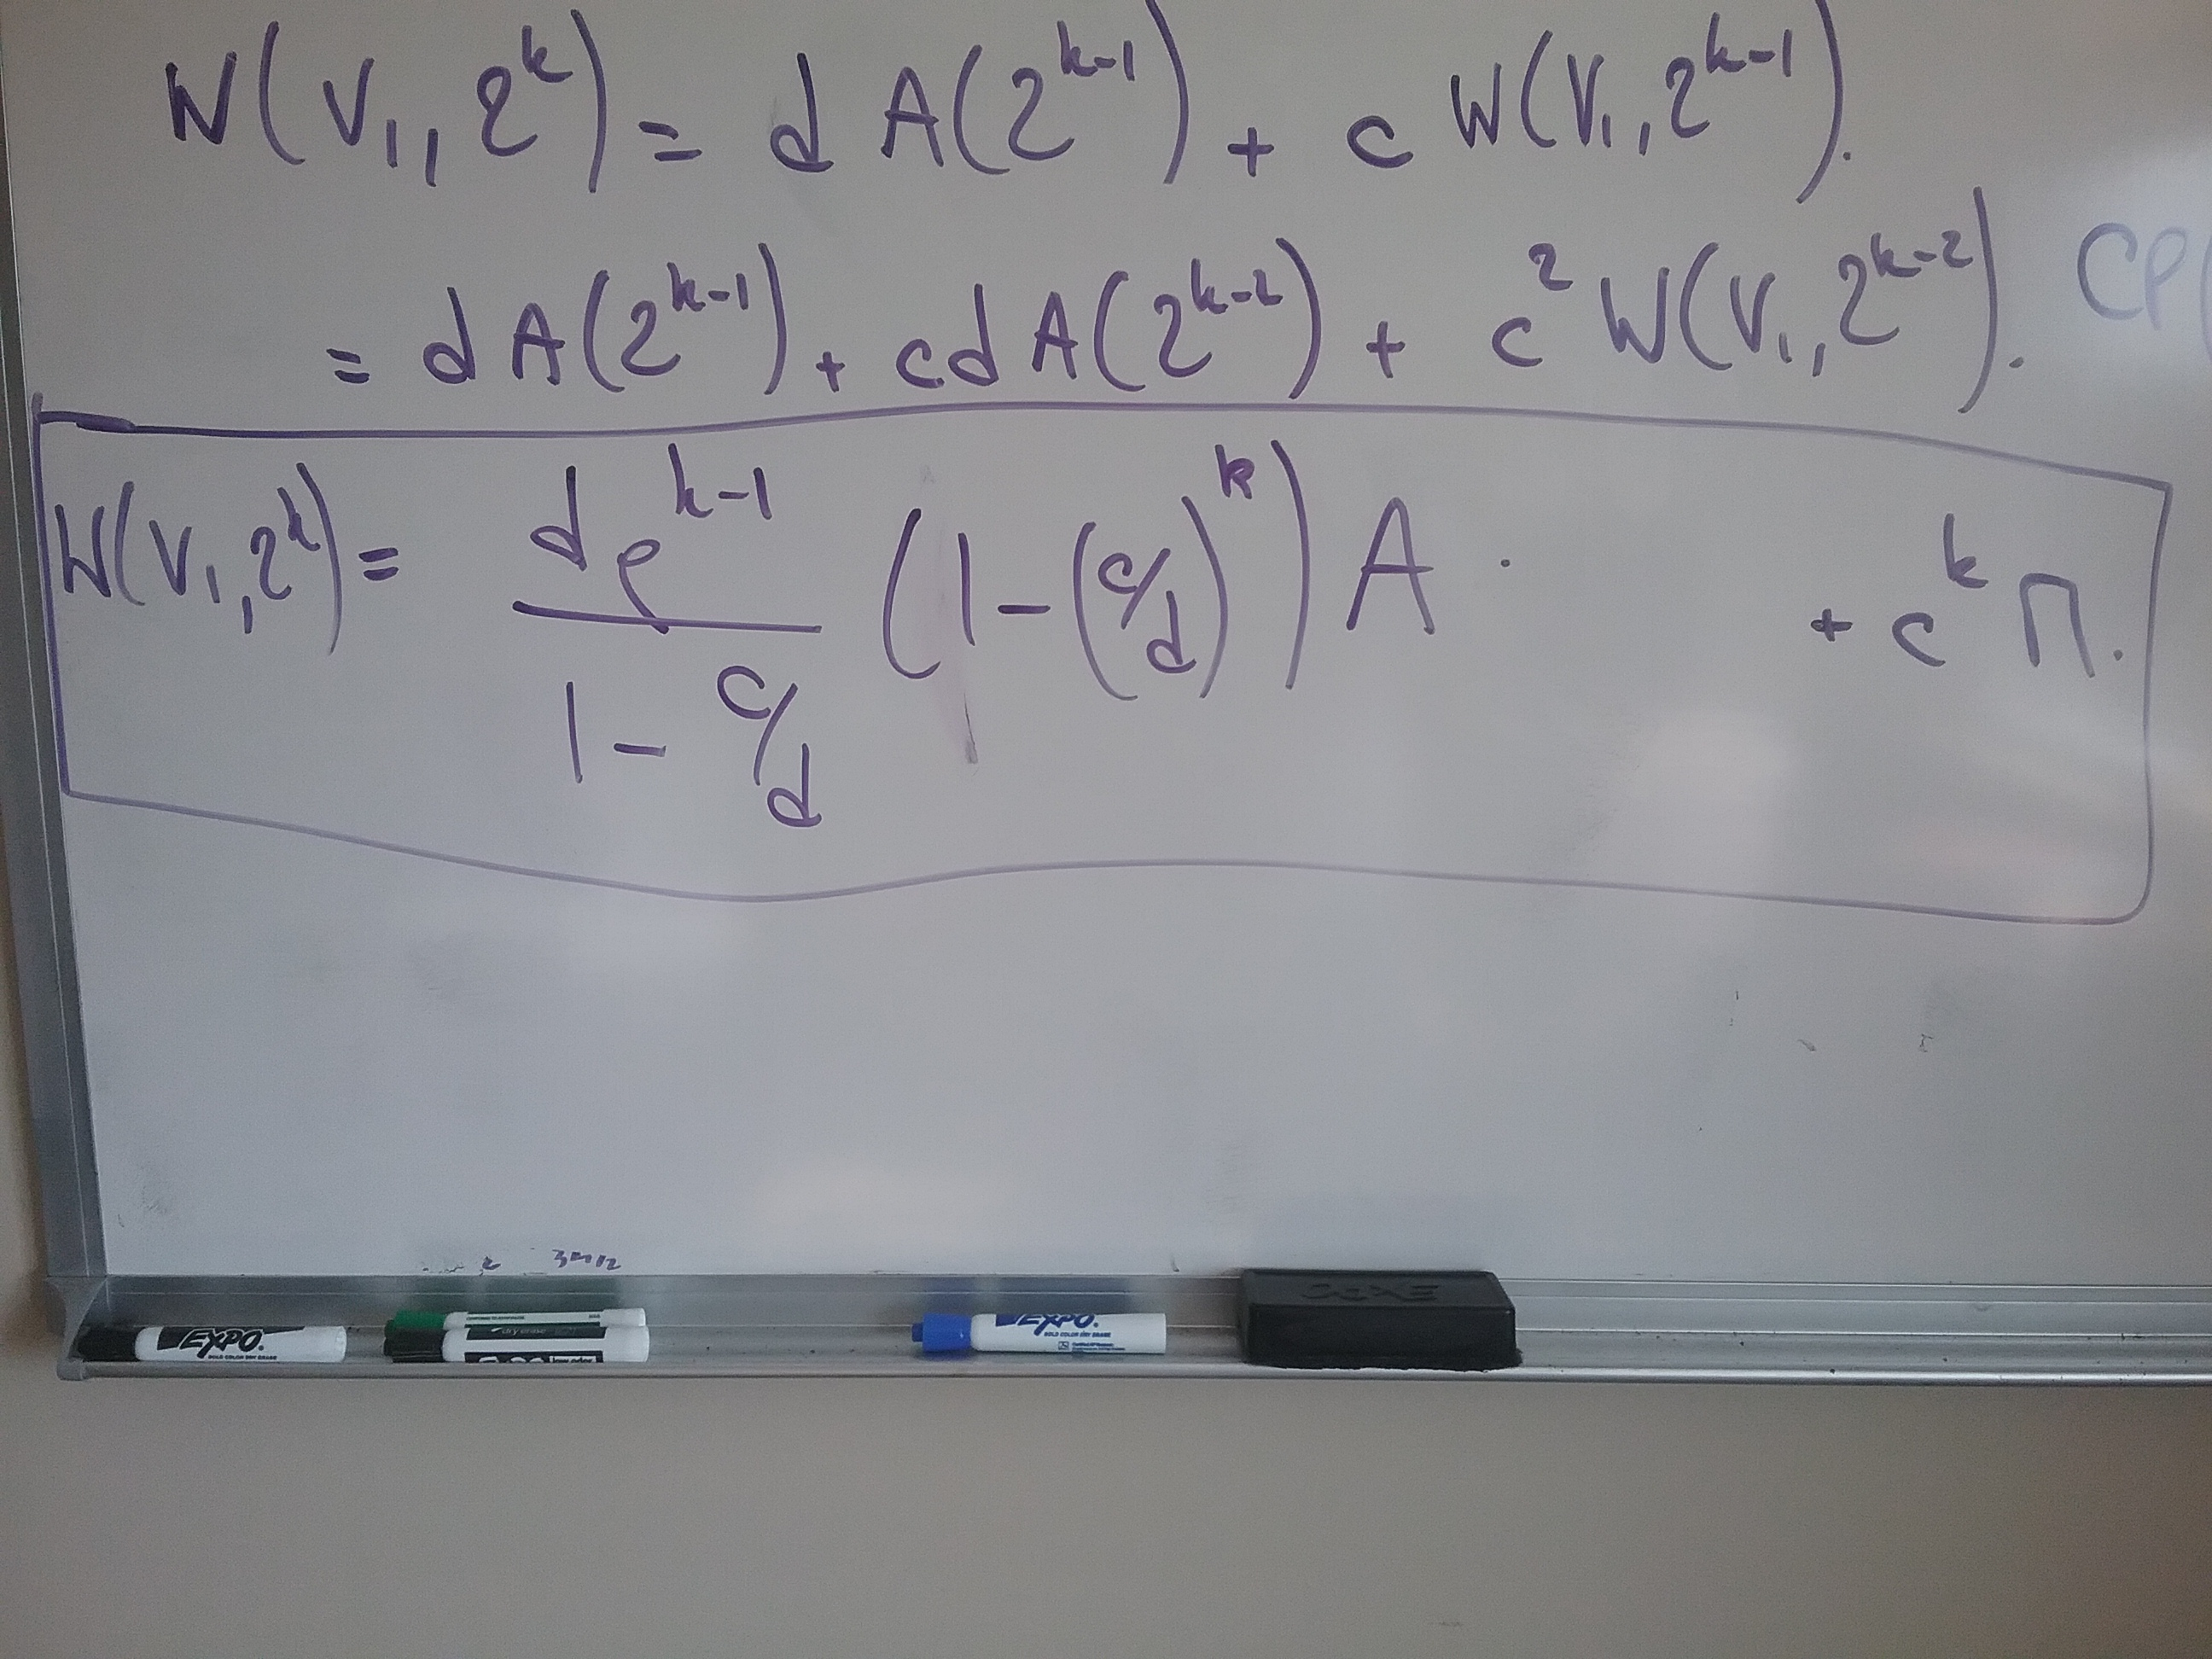
\includegraphics[width=.3\linewidth]{../../notes/20180608_172400.jpg}

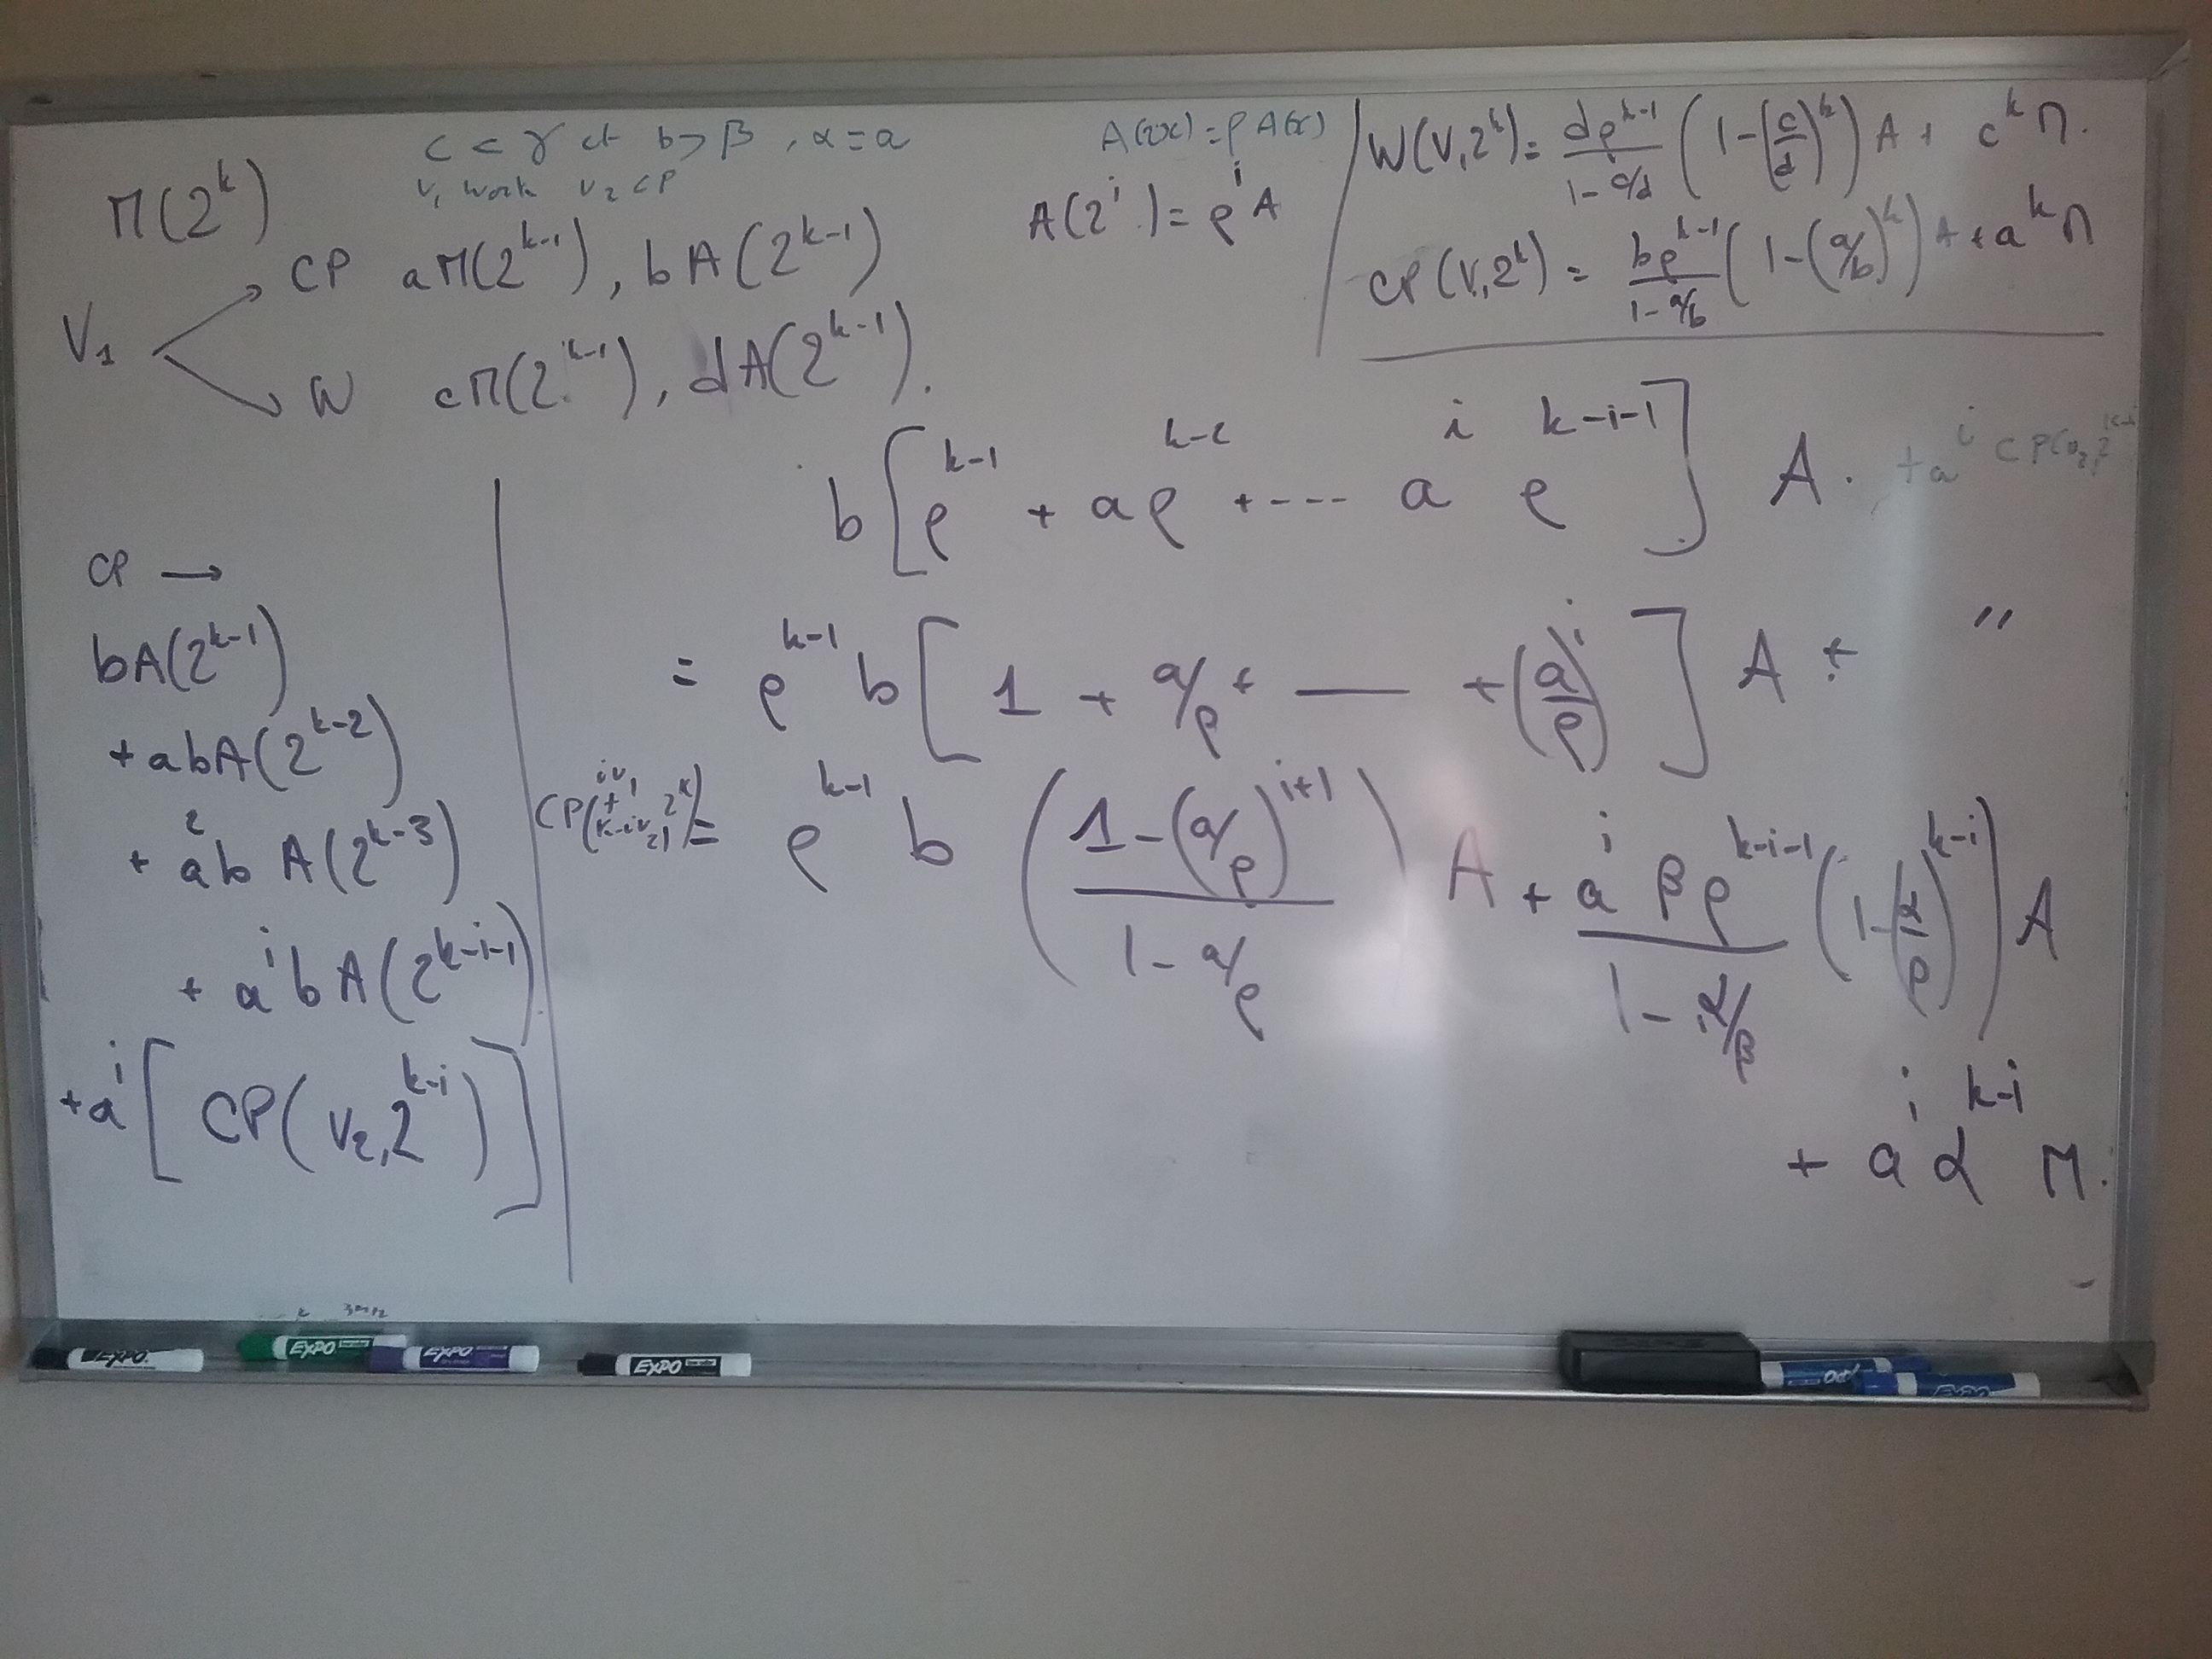
\includegraphics[width=.3\linewidth]{../../notes/20180608_175854.jpg}

\section{MergeSort}

\subsection{Variants}

\subsubsection{Sequential Merge}

\subsubsection{Parallel Merge}

\end{document}
